\chapter{Technische Realisation}

\section{Aufgabenbereiche}

    Welche Komponenten müssen technisch realisiert werden? 


    Siehe Technische Daten

    Beschreibung der prototypischen Realisierung, Vorgehensweise und
    Beschreibung einzelner Schritte


    Beschreibung der prototypischen Realisierung, Vorgehensweise und Beschreibung einzelner Schritte
    Verweise auf das Projekt-Repository in dem weitere Projekt-Artefakte zu finden sind (s.u.).

    \begin{figure}[h]
        \begin{center}
            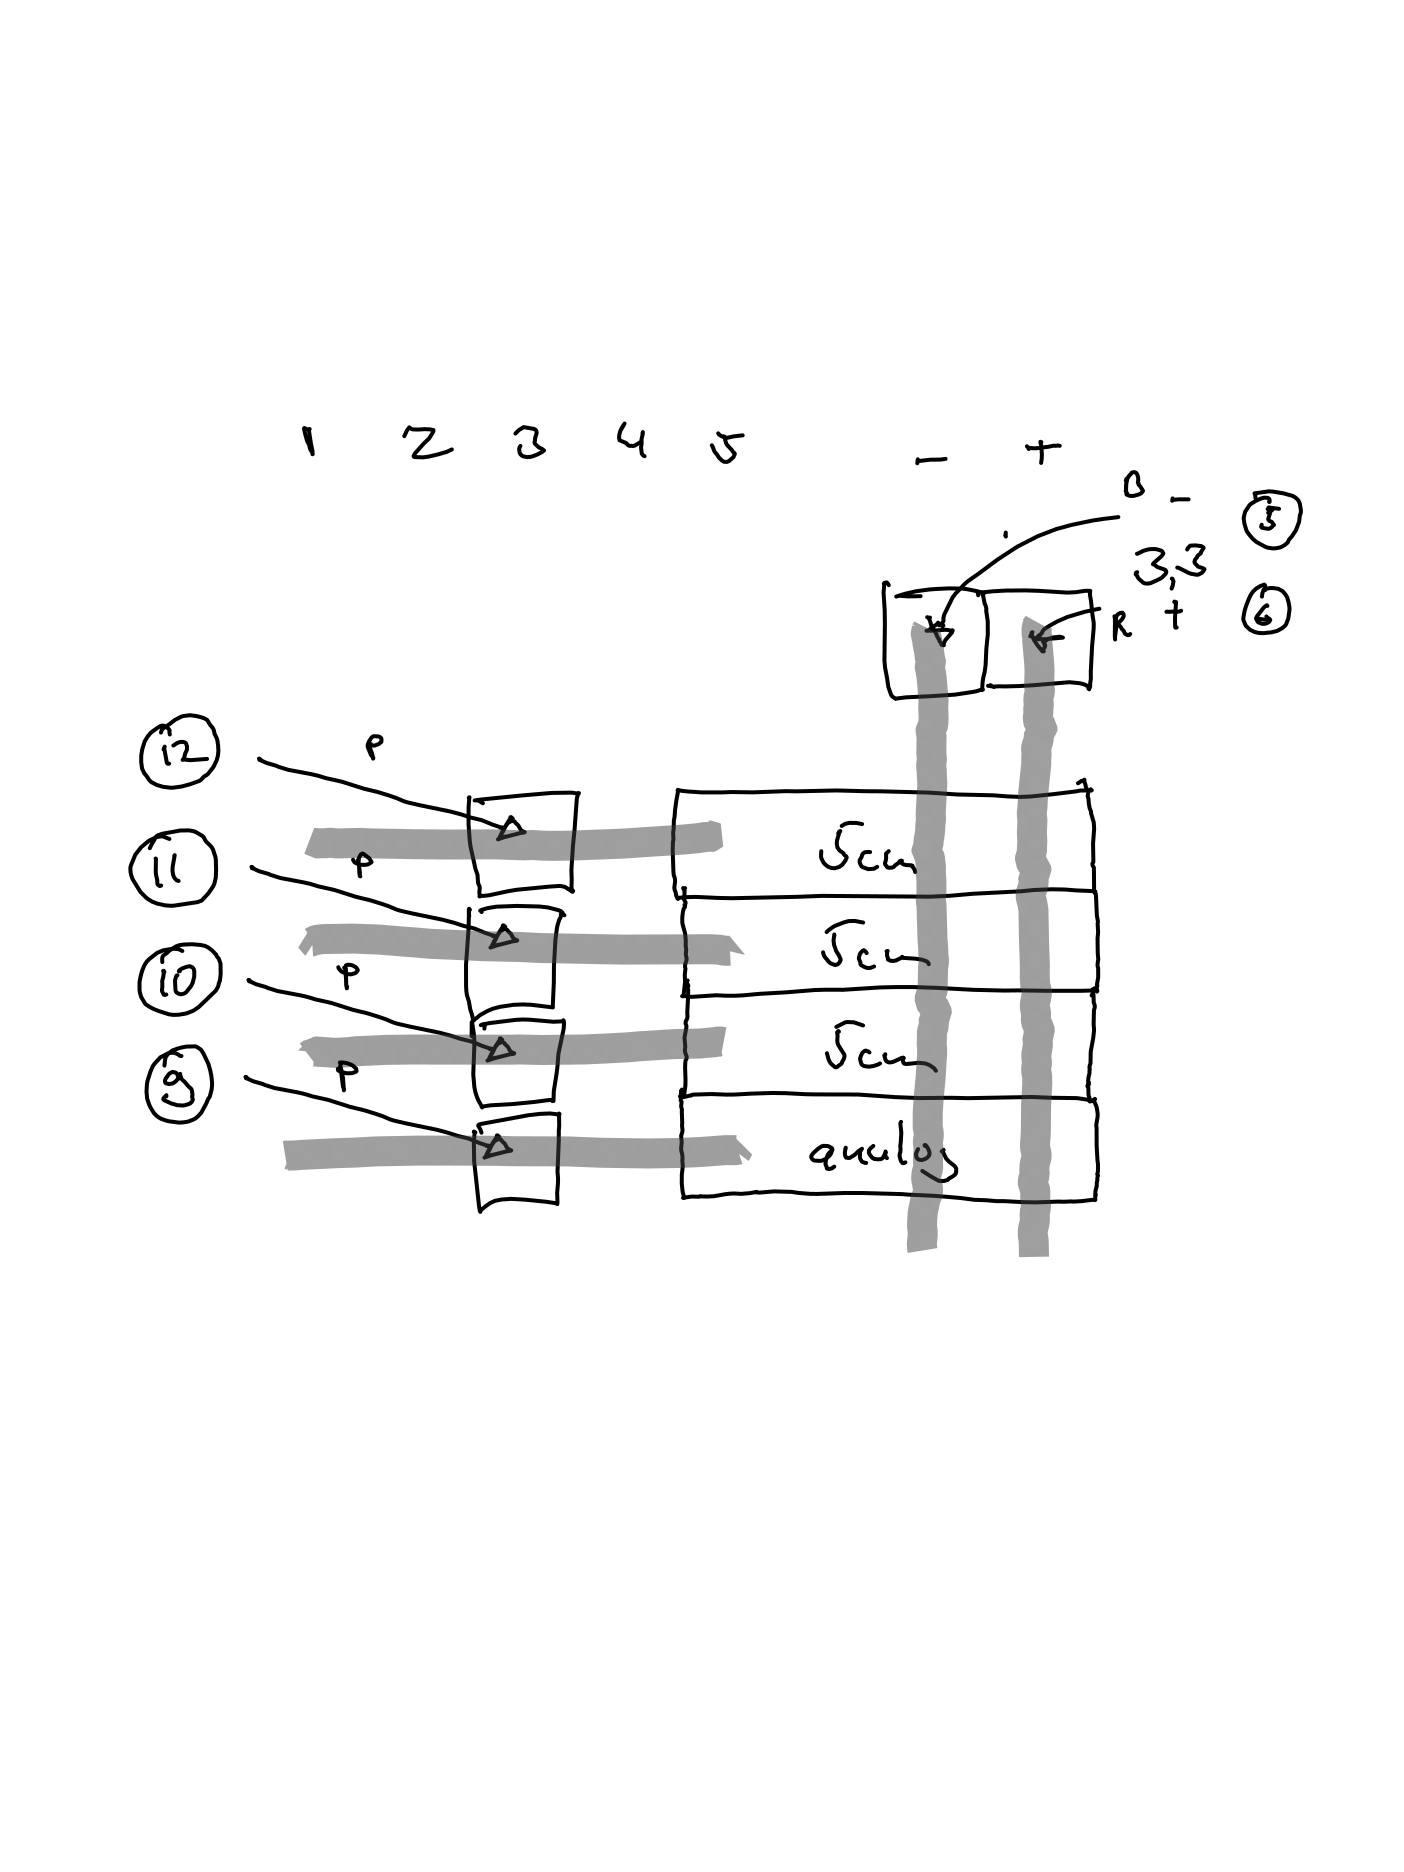
\includegraphics[width=9cm]{media/03_technical_implementation/header_1.png}
        \end{center}
        \caption{Caption}
        \label{fig:header_1}
    \end{figure}

    \begin{figure}[h]
        \begin{center}
            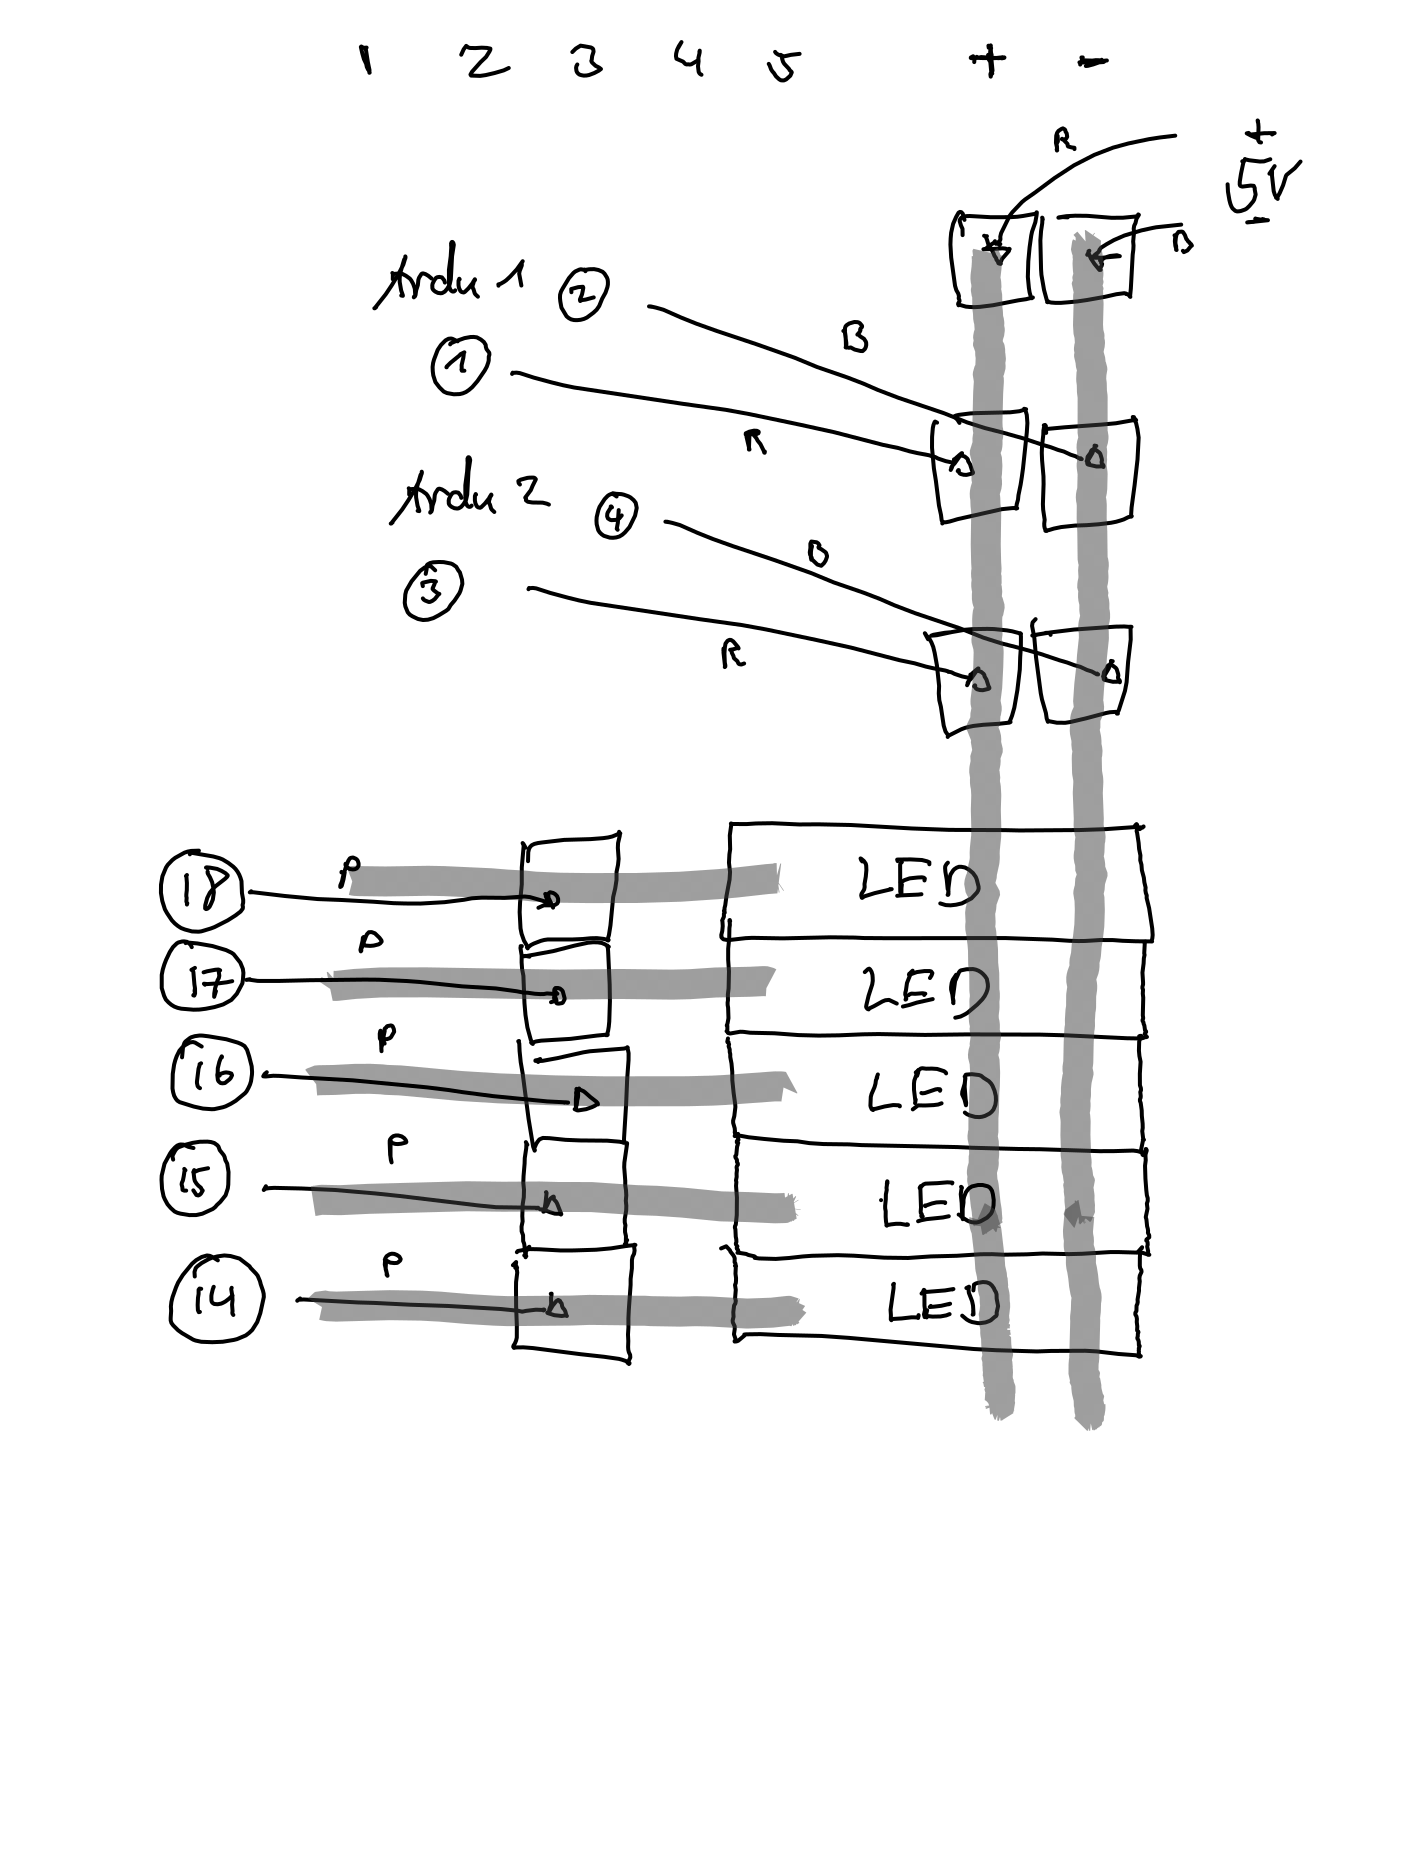
\includegraphics[width=9cm]{media/03_technical_implementation/header_2.png}
        \end{center}
        \caption{Caption}
        \label{fig:header_2}
    \end{figure}



\addtocontents{toc}{\protect\setcounter{tocdepth}{1}}

\section{Mikrocontroller}
    \subsection{Diskussion}
        Warum Arduino

    \subsection{}
        C++ \& PlatformIO

\section{Beleuchtung}
    \subsection{Diskussion}

    \subsection{Implementation}

        \begin{figure}[h]
            \begin{center}
                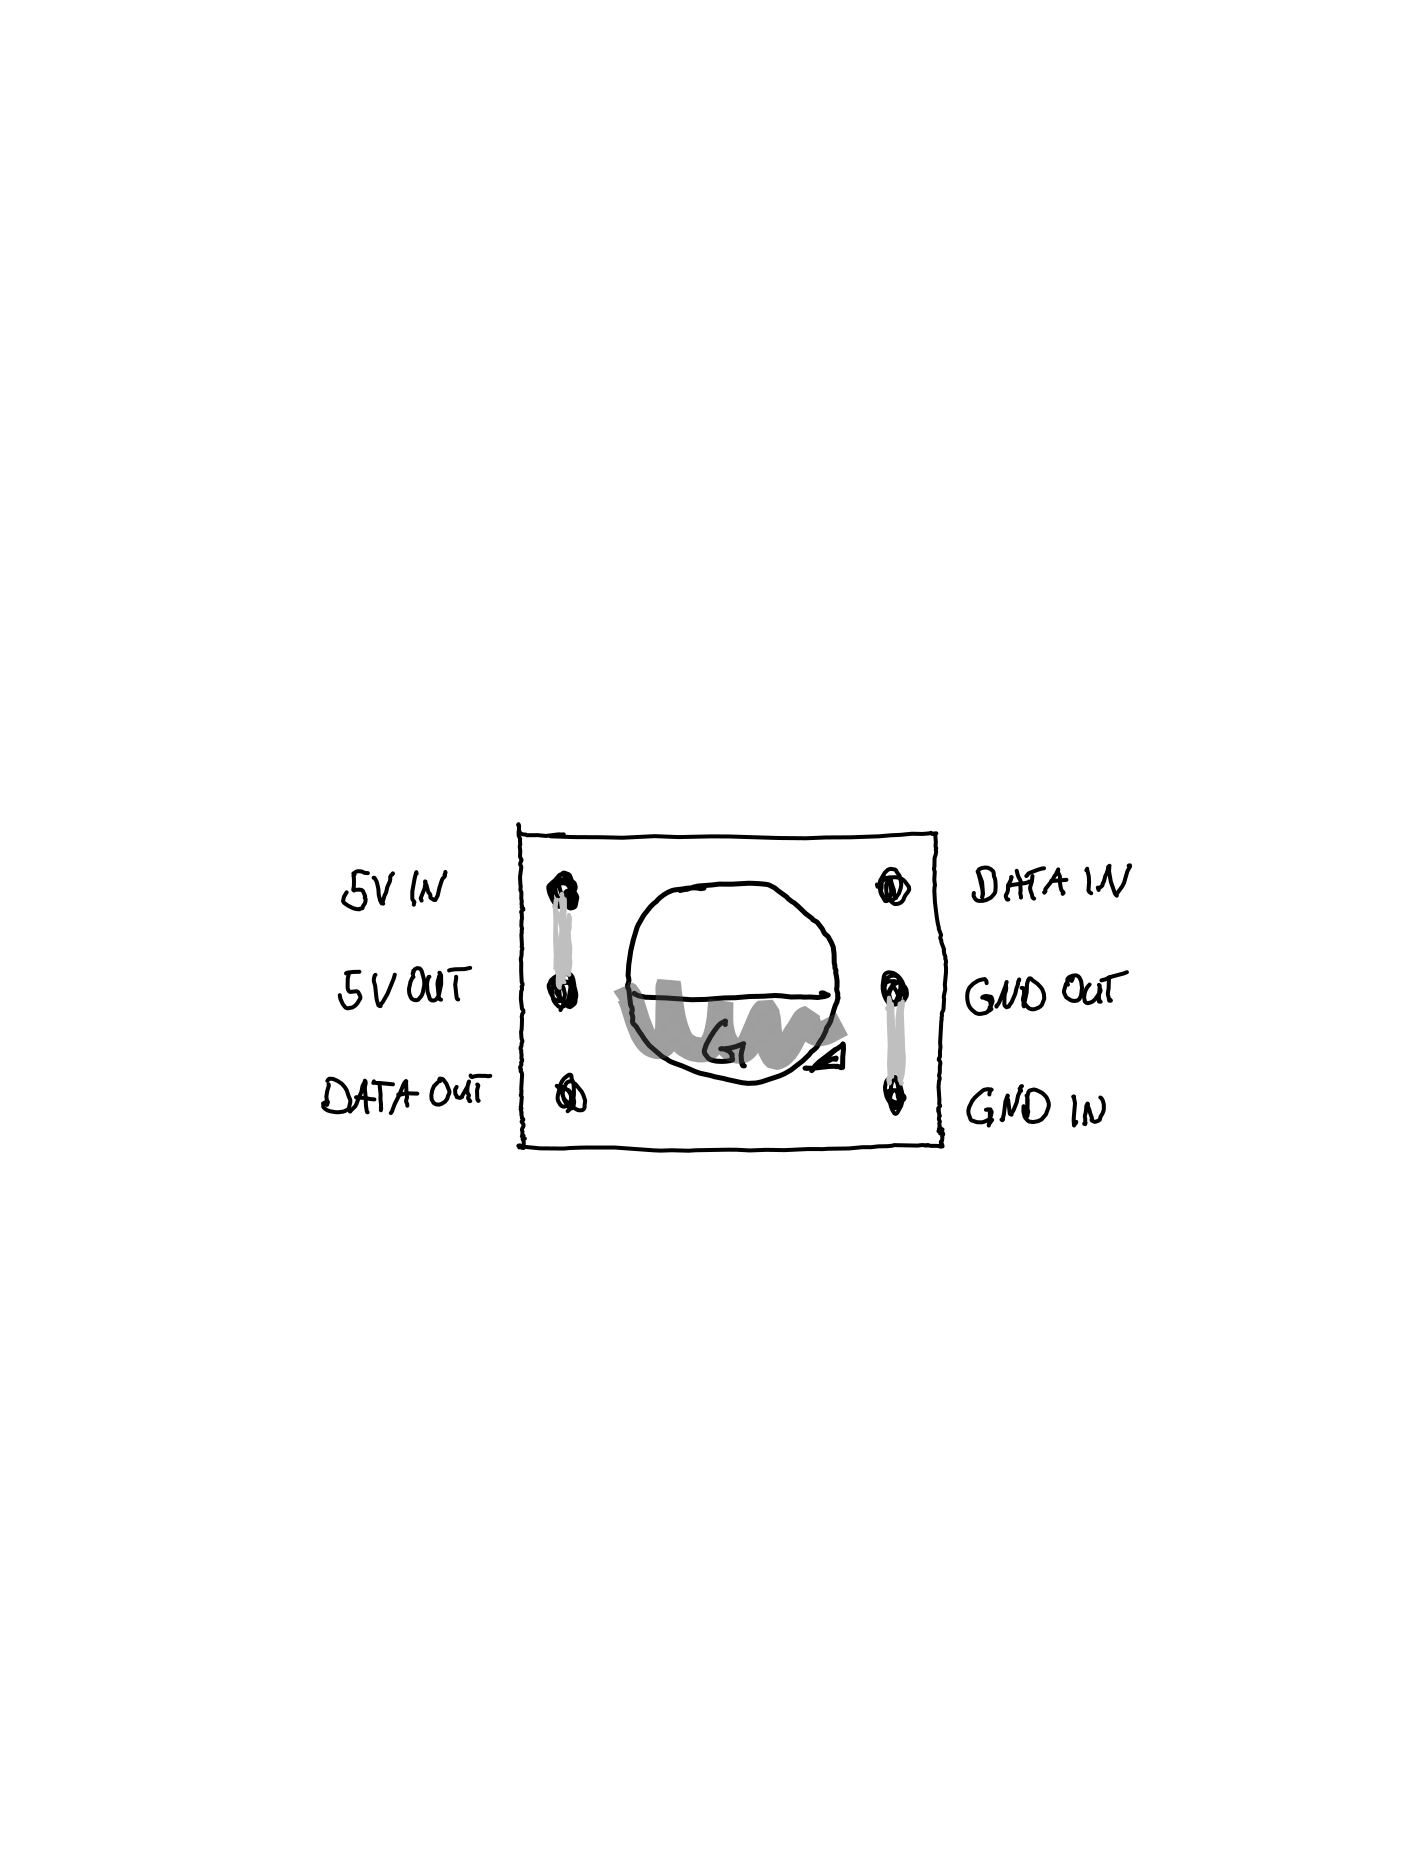
\includegraphics[width=7cm]{media/03_technical_implementation/leds_2.png}
            \end{center}
            \caption{Zeichnung Pin Belegung der NeoPixel SK6812RGBW}
            \label{fig:leds_2}
        \end{figure}
    
        \begin{figure}[h]
            \begin{center}
                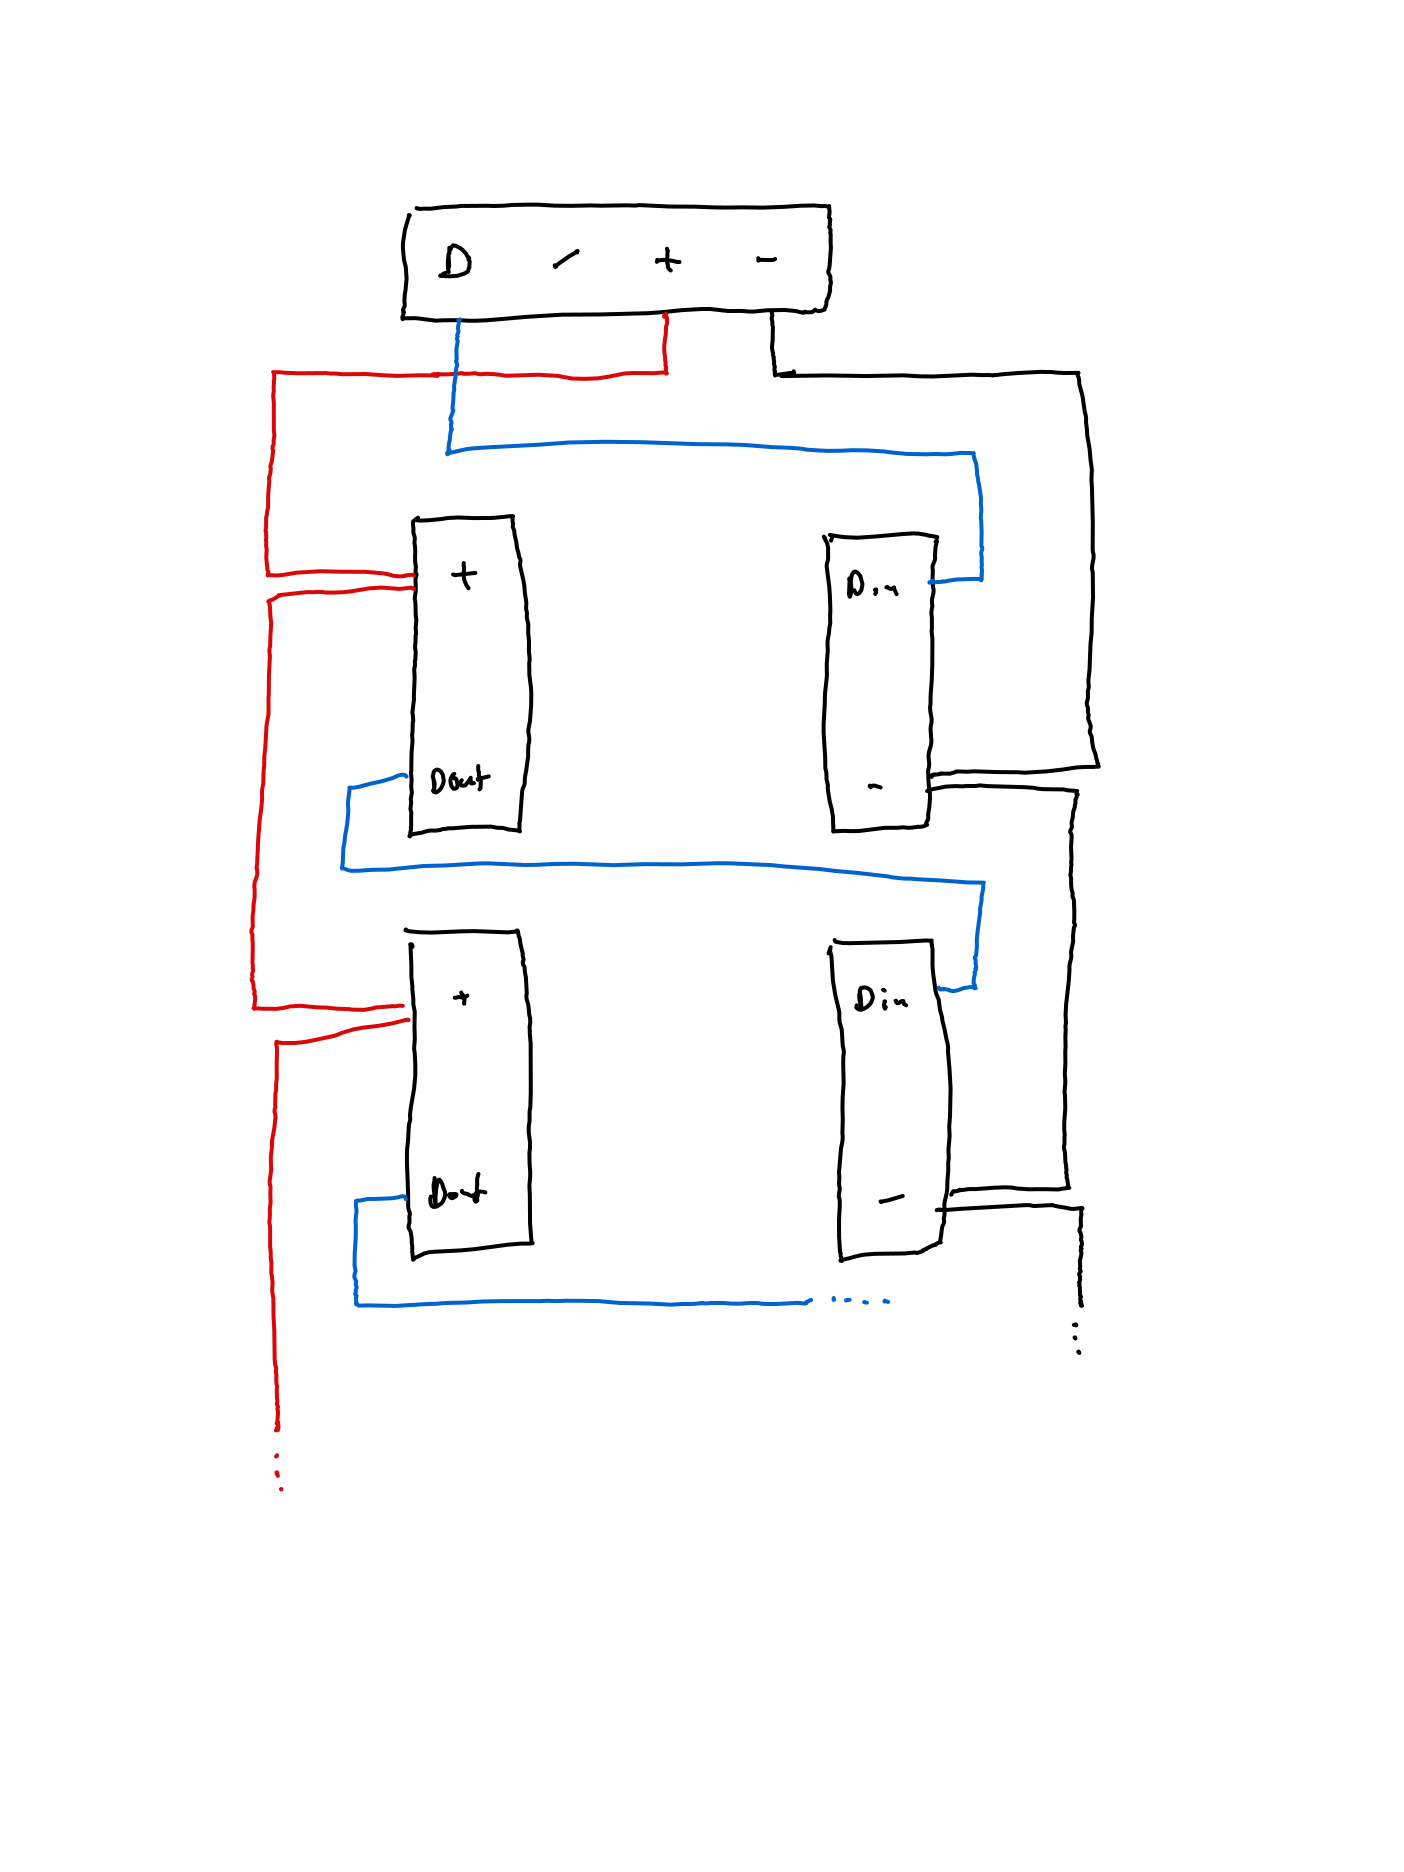
\includegraphics[width=7cm]{media/03_technical_implementation/leds_1.png}
            \end{center}
            \caption{Caption}
            \label{fig:leds_1}
        \end{figure}



\section{Animation}
    \subsection{Diskussion}

    \subsection{Implementation}

\section{Einwurfserkennung}
    \subsection{Diskussion}

    \subsection{Implementation}
        
        \begin{figure}[h]
            \begin{center}
                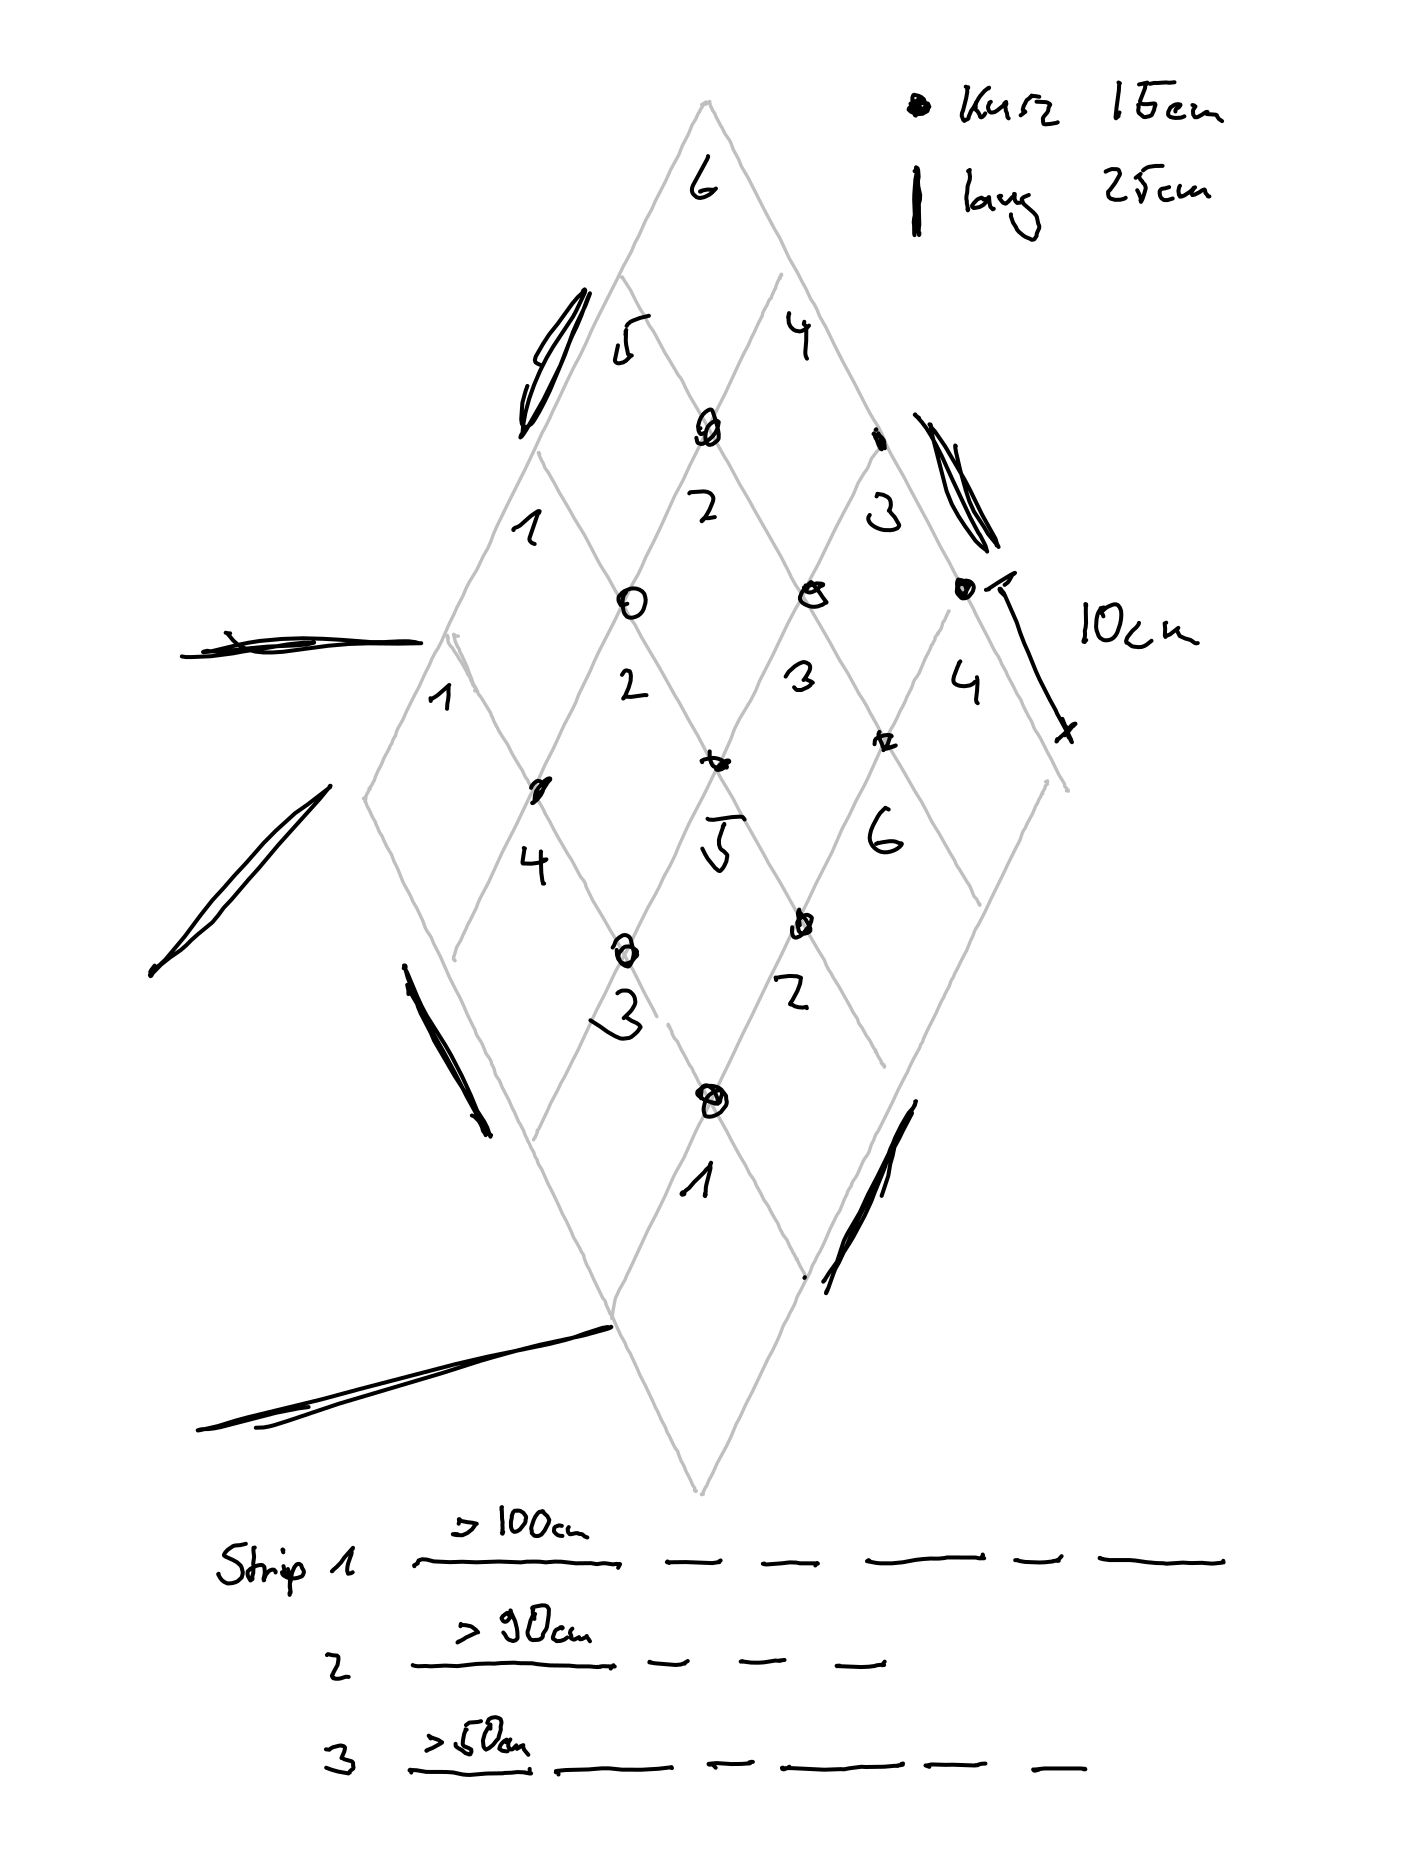
\includegraphics[width=12cm]{media/03_technical_implementation/leds_3.png}
            \end{center}
            \caption{Caption}
            \label{fig:leds_3}
        \end{figure}

\section{Flaschenerkennung (Working Title)}
    \subsection{Diskussion}

    \subsection{Implementation}

\section{Kommunikation zwischen Endgeräten}
    \subsection{Diskussion}

    \subsection{Implementation}

\section{Füllstandsmessung}
    \subsection{Diskussion}

    \subsection{Implementation} 

    \section{Aufgabenbereiche}

\addtocontents{toc}{\protect\setcounter{tocdepth}{2}}

\section{Stückliste}
    siehe Technische Daten.

\section{Zusammenführung von Modell und Technik}
    Der ganze technische Krams und ein bisschen Modellbau
